% -*- coding: utf-8 -*-
% LuaLaTeX 用ドキュメント
% コンパイル: lualatex TowerPathologyExamples.tex

\documentclass[a4paper,11pt]{ltjsarticle}

% LuaTeX-ja 設定
\usepackage{luatexja}
\usepackage{luatexja-fontspec}

% 数学関連
\usepackage{amsmath,amssymb,amsthm}
\usepackage{mathtools}

% 図式・TikZ
\usepackage{tikz}
\usetikzlibrary{arrows.meta,positioning,calc,decorations.pathmorphing,shapes.geometric,patterns}
\usepackage{tikz-cd}

% ハイパーリンク
\usepackage{hyperref}
\hypersetup{
    colorlinks=true,
    linkcolor=blue!70!black,
    urlcolor=blue!50!black
}

% コード表示
\usepackage{listings}
\lstset{
    basicstyle=\ttfamily\small,
    keywordstyle=\color{blue!80!black}\bfseries,
    commentstyle=\color{green!50!black}\itshape,
    stringstyle=\color{red!70!black},
    frame=single,
    breaklines=true,
    numbers=left,
    numberstyle=\tiny\color{gray},
    xleftmargin=2em,
    framexleftmargin=1.5em,
    backgroundcolor=\color{gray!5}
}

% 色
\usepackage{xcolor}

% 定理環境
\theoremstyle{definition}
\newtheorem{definition}{定義}[section]
\newtheorem{example}[definition]{例}
\newtheorem{nonexample}[definition]{非例}
\newtheorem{counterexample}[definition]{反例}

\theoremstyle{plain}
\newtheorem{theorem}[definition]{定理}
\newtheorem{proposition}[definition]{命題}
\newtheorem{lemma}[definition]{補題}

\theoremstyle{remark}
\newtheorem{remark}[definition]{注意}

% カスタムコマンド
\newcommand{\N}{\mathbb{N}}
\newcommand{\Z}{\mathbb{Z}}
\newcommand{\Layer}{\mathrm{layer}}
\newcommand{\minLayer}{\mathrm{minLayer}}
\newcommand{\rank}{\mathrm{rank}}

% タイトル
\title{%
    \textbf{構造塔の病的例と反例}\\[0.5em]
    \Large StructureTowerWithMin の公理の限界を探る
}

\author{su\thanks{Lean ソースコードおよび本 \TeX 文書ともに AI ツール Antigravity (Google DeepMind) を使用して作成しました。}}

\date{2025年12月26日}

\begin{document}

\maketitle

\begin{abstract}
本文書は、構造塔（Structure Tower）理論における病的例・境界例・反例を体系的に解説する。
構造塔は carrier（担体集合）と層（layer）からなる数学的構造であり、
rank（ランク）と minLayer（最小層）の対応を通じて対象の「複雑さ」を階層化する。
本稿では、正常な例との対比において、公理の一つが壊れる例や、
ほぼ公理を満たすが微妙に失敗する例を示し、理論の限界と各公理の必要性を明確化する。
\end{abstract}

\tableofcontents

\newpage

%=============================================================================
\section{導入：構造塔とは何か}
%=============================================================================

\subsection{基本定義}

\begin{definition}[構造塔]
\textbf{構造塔}（Structure Tower）とは、以下のデータの組 $(X, I, \Layer, \minLayer)$ である：
\begin{itemize}
    \item $X$：\textbf{carrier}（担体集合）
    \item $I$：\textbf{Index}（添字集合）、順序集合 $(I, \leq)$
    \item $\Layer : I \to \mathcal{P}(X)$：各添字に対して $X$ の部分集合を対応させる\textbf{層写像}
    \item $\minLayer : X \to I$：各元に対してその\textbf{最小層}を対応させる写像
\end{itemize}
\end{definition}

\begin{definition}[構造塔の公理]
構造塔が well-defined であるためには、以下の3つの公理を満たす必要がある：

\begin{enumerate}
    \item \textbf{被覆性（Covering）}：
    \[
        \forall x \in X,\ \exists i \in I,\ x \in \Layer(i)
    \]
    すべての元は少なくとも一つの層に属する。
    
    \item \textbf{単調性（Monotonicity）}：
    \[
        \forall i, j \in I,\ i \leq j \implies \Layer(i) \subseteq \Layer(j)
    \]
    添字が増えれば層も包含関係で大きくなる。
    
    \item \textbf{最小性（Minimality）}：
    \[
        \forall x \in X,\ x \in \Layer(\minLayer(x)) \land 
        \left( \forall i \in I,\ x \in \Layer(i) \implies \minLayer(x) \leq i \right)
    \]
    minLayer は $x$ が属する層の中で最小のものを返す。
\end{enumerate}
\end{definition}

\subsection{本文書の目的}

正常な構造塔の例だけでなく、\textbf{病的な例}を研究することで、
各公理がなぜ必要なのか、どのような条件で理論が破綻するのかを理解する。

%=============================================================================
\section{例のラベル体系}
%=============================================================================

本稿で使用するラベルの分類を図式で示す。

\begin{figure}[htbp]
\centering
\begin{tikzpicture}[
    node distance=1.5cm and 2cm,
    every node/.style={align=center},
    category/.style={
        rectangle, rounded corners, draw=blue!70!black, 
        fill=blue!10, minimum width=2.8cm, minimum height=1cm,
        font=\small\bfseries
    },
    subcategory/.style={
        rectangle, rounded corners, draw=gray!70, 
        fill=gray!10, minimum width=2.5cm, minimum height=0.8cm,
        font=\small
    },
    arrow/.style={-Stealth, thick, gray!70}
]
% カテゴリノード
\node[category] (trivial) {Trivial};
\node[category, right=of trivial] (canonical) {Canonical};
\node[category, right=of canonical] (extreme) {Extreme};

\node[category, below=1.2cm of trivial] (pathological) {Pathological};
\node[category, right=of pathological] (counter) {Counterexample};
\node[category, right=of counter] (dual) {Dual};

\node[category, below=1.2cm of pathological] (borderline) {Borderline};
\node[category, right=of borderline] (nonexample) {Non-example};
\node[category, right=of nonexample] (schema) {Schema};

% 正常/異常の区分線
\draw[dashed, red!70, thick] 
    ($(trivial.south west) + (-0.3,-0.5)$) -- ($(extreme.south east) + (0.3,-0.5)$)
    node[right, red!70, font=\small] {公理成立};

\draw[dashed, orange!70, thick] 
    ($(borderline.south west) + (-0.3,-0.5)$) -- ($(schema.south east) + (0.3,-0.5)$)
    node[right, orange!70, font=\small] {公理不成立};

\end{tikzpicture}
\caption{例のラベル体系と公理成立の境界}
\label{fig:label-system}
\end{figure}

%=============================================================================
\section{病的例 1：非単調塔（NonMonotoneTower）}
%=============================================================================

\subsection{定義}

\begin{nonexample}[非単調塔]
carrier $X = \N$、添字集合 $I = \N$ に対して、層写像を以下のように定義する：
\[
    \Layer(n) = 
    \begin{cases}
        \emptyset & \text{if } n = 1 \\
        \{k \in \N \mid k \leq n\} & \text{otherwise}
    \end{cases}
\]
\end{nonexample}

\begin{figure}[htbp]
\centering
\begin{tikzpicture}[
    layer/.style={draw=blue!70, fill=blue!10, minimum width=4cm, minimum height=0.8cm},
    empty/.style={draw=red!70, fill=red!10, minimum width=4cm, minimum height=0.8cm, pattern=north east lines, pattern color=red!30},
    elem/.style={circle, draw=black!70, fill=white, minimum size=0.5cm, font=\small}
]

% 層のラベル
\node at (-3, 3) {層};
\node at (0, 3.8) {内容};

% Layer 0
\node[layer] (l0) at (0, 2.4) {};
\node[left=0.5cm of l0] {$\Layer(0)$};
\node[elem] at (-1.2, 2.4) {0};

% Layer 1 (empty - pathological!)
\node[empty] (l1) at (0, 1.2) {};
\node[left=0.5cm of l1] {$\Layer(1)$};
\node[red!70, font=\bfseries] at (0, 1.2) {$\emptyset$ \textbf{(空!)}};

% Layer 2
\node[layer] (l2) at (0, 0) {};
\node[left=0.5cm of l2] {$\Layer(2)$};
\node[elem] at (-1.2, 0) {0};
\node[elem] at (-0.4, 0) {1};
\node[elem] at (0.4, 0) {2};

% Layer 3
\node[layer] (l3) at (0, -1.2) {};
\node[left=0.5cm of l3] {$\Layer(3)$};
\node[elem] at (-1.5, -1.2) {0};
\node[elem] at (-0.7, -1.2) {1};
\node[elem] at (0.1, -1.2) {2};
\node[elem] at (0.9, -1.2) {3};

% 矢印で単調性の失敗を示す
\draw[-Stealth, red!70, thick, dashed] 
    (l0.south) -- (l1.north) 
    node[midway, right, red!70, font=\small] {$\not\subseteq$};

% 説明
\node[font=\small] at (5, 1.8) {$0 \leq 1$ だが};
\node[font=\small] at (5, 1.2) {$\Layer(0) = \{0\} \not\subseteq \emptyset = \Layer(1)$};
\node[red!70, font=\small\bfseries] at (5, 0.5) {単調性が壊れている！};

\end{tikzpicture}
\caption{非単調塔：$\Layer(1) = \emptyset$ により単調性が失敗}
\label{fig:non-monotone}
\end{figure}

\subsection{Lean による形式化}

\begin{lstlisting}[language=ML, caption={非単調塔の Lean 実装}]
/-- 非単調な「塔もどき」の層定義 -/
def nonMonotoneLayer (n : ℕ) : Set ℕ :=
  if n = 1 then ∅ else {k | k ≤ n}

/-- 単調性が壊れていることの証明 -/
theorem nonMonotoneLayer_fails_monotone :
    ¬ (∀ {i j : ℕ}, i ≤ j → nonMonotoneLayer i ⊆ nonMonotoneLayer j) := by
  intro h
  have h01 : nonMonotoneLayer 0 ⊆ nonMonotoneLayer 1 := h (Nat.zero_le 1)
  have h0_in_layer0 : (0 : ℕ) ∈ nonMonotoneLayer 0 := by simp [nonMonotoneLayer]
  have h0_in_layer1 : (0 : ℕ) ∈ nonMonotoneLayer 1 := h01 h0_in_layer0
  simp [nonMonotoneLayer] at h0_in_layer1
\end{lstlisting}

\subsection{数学的解説}

\begin{theorem}
非単調塔は単調性公理を満たさない。具体的には：
\[
    0 \leq 1 \quad \text{かつ} \quad \Layer(0) \not\subseteq \Layer(1)
\]
\end{theorem}

\begin{proof}
$\Layer(0) = \{k \in \N \mid k \leq 0\} = \{0\}$ である。
一方、$\Layer(1) = \emptyset$ と定義されている。
$\{0\} \subseteq \emptyset$ は偽なので、単調性が壊れている。
\end{proof}

\begin{remark}
この例は「層が一時的に消える」ケースを示している。
実際の応用では、フィルトレーションが一時的に縮小するような状況
（例：情報の忘却）をモデル化しようとすると、
構造塔の枠組みでは扱えないことを意味する。
\end{remark}

%=============================================================================
\section{病的例 2：非被覆塔（NonCoveringTower）}
%=============================================================================

\subsection{定義}

\begin{nonexample}[非被覆塔]
carrier $X = \N$、添字集合 $I = \N$ に対して、層写像を以下のように定義する：
\[
    \Layer(n) = \{k \in \N \mid k \leq n \land k \neq 0\}
\]
すなわち、$0$ を意図的に除外した層である。
\end{nonexample}

\begin{figure}[htbp]
\centering
\begin{tikzpicture}[
    layer/.style={draw=blue!70, fill=blue!10, minimum width=5cm, minimum height=0.8cm},
    elem/.style={circle, draw=black!70, fill=white, minimum size=0.5cm, font=\small},
    orphan/.style={circle, draw=red!70, fill=red!10, minimum size=0.6cm, font=\small\bfseries}
]

% 「孤児」の 0
\node[orphan] (zero) at (-3.5, 0.6) {0};
\node[red!70, font=\small] at (-3.5, -0.1) {どの層にも};
\node[red!70, font=\small] at (-3.5, -0.5) {属さない！};

% 層
\node[layer] (l0) at (1.5, 2.4) {};
\node[left=0.3cm of l0] {$\Layer(0)$};
\node[gray] at (1.5, 2.4) {$\emptyset$};

\node[layer] (l1) at (1.5, 1.2) {};
\node[left=0.3cm of l1] {$\Layer(1)$};
\node[elem] at (1.5, 1.2) {1};

\node[layer] (l2) at (1.5, 0) {};
\node[left=0.3cm of l2] {$\Layer(2)$};
\node[elem] at (0.7, 0) {1};
\node[elem] at (1.5, 0) {2};

\node[layer] (l3) at (1.5, -1.2) {};
\node[left=0.3cm of l3] {$\Layer(3)$};
\node[elem] at (0.3, -1.2) {1};
\node[elem] at (1.1, -1.2) {2};
\node[elem] at (1.9, -1.2) {3};

% 赤い X で 0 が含まれないことを強調
\draw[red!70, thick] (zero.north west) -- (zero.south east);
\draw[red!70, thick] (zero.north east) -- (zero.south west);

% 説明
\node[text width=4.5cm, align=left, font=\small] at (5.5, 1.2) {被覆性の失敗：};
\node[font=\small] at (5.5, 0.6) {$\forall n \in \N,\ 0 \notin \Layer(n)$};
\node[red!70, font=\small\bfseries] at (5.5, 0) {0 は「孤児」になる};

% 単調性は OK の注釈
\node[green!50!black, font=\small] at (1.5, -2) {※ 単調性は成立};
\node[green!50!black, font=\small] at (1.5, -2.5) {$\Layer(i) \subseteq \Layer(j)$ for $i \leq j$};

\end{tikzpicture}
\caption{非被覆塔：$0$ はどの層にも属さない}
\label{fig:non-covering}
\end{figure}

\subsection{Lean による形式化}

\begin{lstlisting}[language=ML, caption={非被覆塔の Lean 実装}]
/-- 0 を含まない「塔もどき」の層定義 -/
def noCoveringLayer (n : ℕ) : Set ℕ :=
  {k | k ≤ n ∧ k ≠ 0}

/-- 0 がどの層にも属さないことを示す -/
theorem zero_not_in_any_noCoveringLayer :
    ∀ n : ℕ, (0 : ℕ) ∉ noCoveringLayer n := by
  intro n
  simp [noCoveringLayer]

/-- covering 公理が壊れていることの証明 -/
theorem noCoveringLayer_fails_covering :
    ¬ (∀ x : ℕ, ∃ i : ℕ, x ∈ noCoveringLayer i) := by
  push_neg
  refine ⟨0, ?_⟩
  intro i
  exact zero_not_in_any_noCoveringLayer i

/-- 単調性は成立することを確認 -/
theorem noCoveringLayer_monotone :
    ∀ {i j : ℕ}, i ≤ j → noCoveringLayer i ⊆ noCoveringLayer j := by
  intro i j hij x hx
  simp [noCoveringLayer] at hx ⊢
  exact ⟨le_trans hx.1 hij, hx.2⟩
\end{lstlisting}

\subsection{数学的解説}

\begin{theorem}
非被覆塔は被覆性公理を満たさない。具体的には：
\[
    \nexists i \in \N,\ 0 \in \Layer(i)
\]
\end{theorem}

\begin{proof}
任意の $n \in \N$ に対して、$\Layer(n) = \{k \mid k \leq n \land k \neq 0\}$ である。
$0 \neq 0$ は偽なので、$0 \in \Layer(n)$ は任意の $n$ で偽。
\end{proof}

\begin{proposition}
非被覆塔は単調性公理を満たす。
\end{proposition}

\begin{proof}
$i \leq j$ とする。$x \in \Layer(i)$ ならば $x \leq i \land x \neq 0$。
$i \leq j$ より $x \leq j$ なので、$x \leq j \land x \neq 0$、すなわち $x \in \Layer(j)$。
\end{proof}

\begin{remark}
この例は「公理の独立性」を示している。
単調性を満たしても被覆性を満たさない構造が存在し、
両公理は論理的に独立である。
\end{remark}

%=============================================================================
\section{正規形との比較：正常な自然数塔}
%=============================================================================

\subsection{定義}

\begin{example}[自然数塔（Canonical）]
carrier $X = \N$、添字集合 $I = \N$ に対して：
\begin{align*}
    \Layer(n) &= \{k \in \N \mid k \leq n\} \\
    \minLayer(x) &= x
\end{align*}
この塔は $\rank \equiv \minLayer$ の\textbf{正規形}（canonical form）である。
\end{example}

\begin{figure}[htbp]
\centering
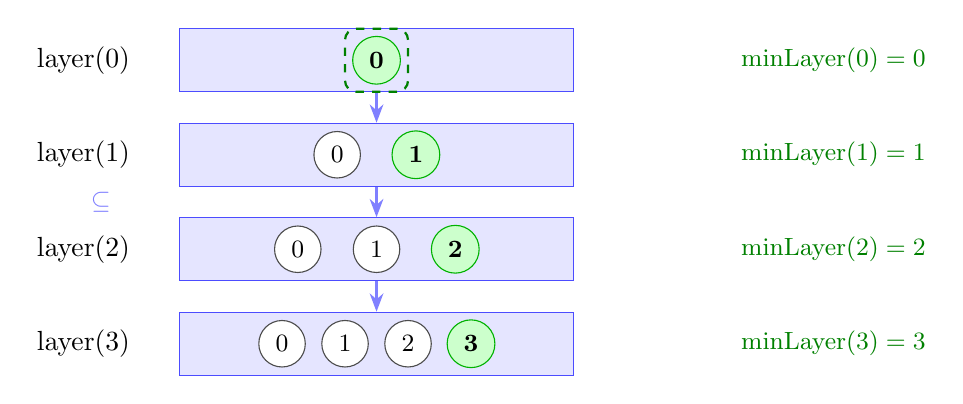
\begin{tikzpicture}[
    layer/.style={draw=blue!70, fill=blue!10, minimum width=5cm, minimum height=0.8cm},
    elem/.style={circle, draw=black!70, fill=white, minimum size=0.5cm, font=\small},
    highlight/.style={circle, draw=green!70!black, fill=green!20, minimum size=0.6cm, font=\small\bfseries}
]

% 層
\node[layer] (l0) at (0, 3) {};
\node[left=0.5cm of l0] {$\Layer(0)$};
\node[highlight] at (0, 3) {0};
\node[right=2cm of l0, green!50!black, font=\small] {$\minLayer(0) = 0$};

\node[layer] (l1) at (0, 1.8) {};
\node[left=0.5cm of l1] {$\Layer(1)$};
\node[elem] at (-0.5, 1.8) {0};
\node[highlight] at (0.5, 1.8) {1};
\node[right=2cm of l1, green!50!black, font=\small] {$\minLayer(1) = 1$};

\node[layer] (l2) at (0, 0.6) {};
\node[left=0.5cm of l2] {$\Layer(2)$};
\node[elem] at (-1, 0.6) {0};
\node[elem] at (0, 0.6) {1};
\node[highlight] at (1, 0.6) {2};
\node[right=2cm of l2, green!50!black, font=\small] {$\minLayer(2) = 2$};

\node[layer] (l3) at (0, -0.6) {};
\node[left=0.5cm of l3] {$\Layer(3)$};
\node[elem] at (-1.2, -0.6) {0};
\node[elem] at (-0.4, -0.6) {1};
\node[elem] at (0.4, -0.6) {2};
\node[highlight] at (1.2, -0.6) {3};
\node[right=2cm of l3, green!50!black, font=\small] {$\minLayer(3) = 3$};

% 包含関係の矢印
\draw[-Stealth, blue!50, thick] (l0.south) -- (l1.north);
\draw[-Stealth, blue!50, thick] (l1.south) -- (l2.north);
\draw[-Stealth, blue!50, thick] (l2.south) -- (l3.north);
\node[blue!50, font=\small] at (-3.5, 1.2) {$\subseteq$};

% 対角線での強調
\draw[green!50!black, thick, dashed, rounded corners] 
    (-0.4, 3.4) -- (0.4, 3.4) -- (0.4, 2.6) -- (-0.4, 2.6) -- cycle;

\end{tikzpicture}
\caption{正常な自然数塔：$\minLayer = \mathrm{id}$ による正規形}
\label{fig:canonical-tower}
\end{figure}

\subsection{公理の検証}

\begin{theorem}
自然数塔はすべての公理を満たす。
\end{theorem}

\begin{proof}
\textbf{被覆性}：任意の $x \in \N$ に対して、$x \in \Layer(x)$（$x \leq x$ より）。

\textbf{単調性}：$i \leq j$ かつ $k \in \Layer(i)$ とする。
$k \leq i \leq j$ より $k \in \Layer(j)$。

\textbf{最小性}：$\minLayer(x) = x$ とおく。
$x \in \Layer(x)$ は $x \leq x$ より成立。
$x \in \Layer(i)$ ならば $x \leq i$ なので $\minLayer(x) = x \leq i$。
\end{proof}

%=============================================================================
\section{計算可能な例：Fin 5 塔}
%=============================================================================

\begin{example}[Fin 5 塔]
有限集合 $X = \{0, 1, 2, 3, 4\}$（Lean では $\mathtt{Fin}\ 5$）に対して：
\begin{align*}
    \Layer(n) &= \{k \in \mathrm{Fin}\ 5 \mid k.\mathrm{val} \leq n\} \\
    \minLayer(k) &= k.\mathrm{val}
\end{align*}
\end{example}

この例は\textbf{完全に計算可能}であり、Lean の \texttt{\#eval} で実行テストが可能である。

\begin{lstlisting}[language=ML, caption={Fin 5 塔の計算テスト}]
#eval fin5MinLayer ⟨0, by omega⟩  -- 結果: 0
#eval fin5MinLayer ⟨3, by omega⟩  -- 結果: 3
#eval fin5MinLayer ⟨4, by omega⟩  -- 結果: 4

#eval decide ((⟨2, by omega⟩ : Fin 5) ∈ fin5Layer 3)   -- true
#eval decide ((⟨4, by omega⟩ : Fin 5) ∈ fin5Layer 3)   -- false
#eval decide ((⟨4, by omega⟩ : Fin 5) ∈ fin5Layer 4)   -- true
\end{lstlisting}

%=============================================================================
\section{例のカタログ（全21例）}
%=============================================================================

以下に、本理論で検討した全21例を分類表としてまとめる。

\begin{table}[htbp]
\centering
\caption{構造塔の例カタログ}
\label{tab:catalog}
\small
\begin{tabular}{|c|l|c|c|c|l|}
\hline
\textbf{番号} & \textbf{名称} & \textbf{被覆} & \textbf{単調} & \textbf{最小} & \textbf{ラベル} \\
\hline
\hline
1 & pointTower & $\checkmark$ & $\checkmark$ & $\checkmark$ & Trivial \\
2 & emptyIndexTower & — & — & — & Trivial \\
\hline
3 & natIdentityTower & $\checkmark$ & $\checkmark$ & $\checkmark$ & Canonical \\
4 & intAbsTower & $\checkmark$ & $\checkmark$ & $\checkmark$ & Canonical \\
\hline
5 & productTower & $\checkmark$ & $\checkmark$ & $\checkmark$ & Extreme \\
6 & infiniteWidthTower & $\checkmark$ & $\checkmark$ & ? & Extreme \\
\hline
7 & \textbf{nonMonotoneTower} & $\checkmark$ & $\times$ & — & \textcolor{red}{Pathological} \\
8 & \textbf{nonCoveringTower} & $\times$ & $\checkmark$ & — & \textcolor{red}{Pathological} \\
\hline
9 & rankNotUniqueTower & $\checkmark$ & $\checkmark$ & $\times$ & Counterexample \\
10 & layerNotSetTower & — & — & — & Counterexample \\
\hline
11 & codepthTower & $\checkmark$ & $\checkmark$ & $\checkmark$ & Dual \\
12 & topologyRefinementTower & $\checkmark$ & $\checkmark$ & $\checkmark$ & Dual \\
\hline
13 & singletonLayerTower & — & $\times$ & — & Borderline \\
14 & thresholdTower & $\checkmark$ & $\checkmark$ & $\checkmark$ & Borderline \\
\hline
15 & partialMinLayer & $\checkmark$ & $\checkmark$ & $\times$ & Non-example \\
16 & multiMinimalTower & $\checkmark$ & $\checkmark$ & $\times$ & Non-example \\
\hline
17 & preSheafTower & — & — & — & Meta \\
18 & gradedModuleTower & $\checkmark$ & $\checkmark$ & $\checkmark$ & Meta \\
\hline
19 & closureOperatorTower & $\checkmark$ & $\checkmark$ & $\checkmark$ & Schema \\
20 & generatedTower & $\checkmark$ & $\checkmark$ & $\checkmark$ & Schema \\
\hline
21 & fin5Tower & $\checkmark$ & $\checkmark$ & $\checkmark$ & Computational \\
\hline
\end{tabular}
\end{table}

%=============================================================================
\section{公理間の依存関係}
%=============================================================================

\begin{figure}[htbp]
\centering
\begin{tikzpicture}[
    axiom/.style={
        rectangle, rounded corners=5pt, draw=blue!70!black, 
        fill=blue!15, minimum width=3cm, minimum height=1.2cm,
        font=\bfseries, text=blue!70!black
    },
    implication/.style={-Stealth, thick, black!60},
    norelation/.style={thick, red!60, dashed}
]
% 公理ノード
\node[axiom] (covering) at (0, 2) {Covering};
\node[axiom] (monotone) at (5, 2) {Monotonicity};
\node[axiom] (minimal) at (2.5, -1) {Minimality};

% 日本語ラベルを下に追加
\node[font=\scriptsize] at (0, 1.2) {(被覆性)};
\node[font=\scriptsize] at (5, 1.2) {(単調性)};
\node[font=\scriptsize] at (2.5, -1.8) {(最小性)};

% 依存矢印
\draw[implication] (covering) -- (minimal) 
    node[midway, left, font=\small] {前提};
\draw[implication] (monotone) -- (minimal) 
    node[midway, right, font=\small] {前提};

% 独立を示す線
\draw[norelation] (covering) -- (monotone)
    node[midway, above, font=\small, red!60] {独立};

% 説明テキスト
\node[font=\small\bfseries] at (2.5, -3) {公理の独立性};
\node[font=\small, text width=8cm, align=left] at (2.5, -4) {• 非単調塔（例7）：被覆OK、単調NG};
\node[font=\small, text width=8cm, align=left] at (2.5, -4.5) {• 非被覆塔（例8）：被覆NG、単調OK};
\node[font=\small, text width=8cm, align=left] at (2.5, -5) {• 最小性は両方を前提とする};

\end{tikzpicture}
\caption{構造塔の公理間の論理的依存関係}
\label{fig:axiom-deps}
\end{figure}

%=============================================================================
\section{結論}
%=============================================================================

本文書では、構造塔理論における病的例・境界例・反例を体系的に分析した。
主な知見は以下の通りである：

\begin{enumerate}
    \item \textbf{公理の必要性}：
    被覆性と単調性は論理的に独立であり、どちらか一方が壊れる例が構成できる。

    \item \textbf{公理の前提関係}：
    最小性（minLayer の well-definedness）は、被覆性と単調性の両方を前提とする。

    \item \textbf{計算可能性}：
    有限の例（Fin 5 塔）では、層所属や minLayer が完全に計算可能であり、
    Lean の \texttt{\#eval} で検証できる。

    \item \textbf{理論の境界}：
    順序が線形でない場合（例9）や、層が部分集合でない場合（例10）は、
    標準的な構造塔の枠組みから外れる。
\end{enumerate}

これらの病的例は、構造塔理論を応用する際に、
どのような仮定が暗黙に置かれているかを明確化する上で重要である。

%=============================================================================
% 参考文献
%=============================================================================

\begin{thebibliography}{9}

\bibitem{mathlib}
The mathlib Community.
\textit{Mathlib: The Math Library for Lean 4}.
\url{https://github.com/leanprover-community/mathlib4}

\bibitem{bourbaki}
N. Bourbaki.
\textit{Éléments de mathématique: Théorie des ensembles}.
Hermann, 1970.

\bibitem{lean4}
Leonardo de Moura et al.
\textit{The Lean 4 Theorem Prover and Programming Language}.
CADE-28, 2021.

\end{thebibliography}

\end{document}
